\documentclass[mat1, tisk]{fmfdelo}
\usepackage{amsmath}
\usepackage{graphicx}
% \documentclass[fin1, tisk]{fmfdelo}
% Če pobrišete možnost tisk, bodo povezave obarvane,
% na začetku pa ne bo praznih strani po naslovu, …

%%%%%%%%%%%%%%%%%%%%%%%%%%%%%%%%%%%%%%%%%%%%%%%%%%%%%%%%%%%%%%%%%%%%%%%%%%%%%%%
% METAPODATKI
%%%%%%%%%%%%%%%%%%%%%%%%%%%%%%%%%%%%%%%%%%%%%%%%%%%%%%%%%%%%%%%%%%%%%%%%%%%%%%%

% - vaše ime
\avtor{Manca Murn}

% - naslov dela v slovenščini
\naslov{Metrična dimenzija leksikografskega produkta grafov}

% - naslov dela v angleščini
\title{The metric dimension of the lexicographic product of graphs}

% - ime mentorja/mentorice s polnim nazivom:
%   - doc.~dr.~Ime Priimek
%   - izr.~prof.~dr.~Ime Priimek
%   - prof.~dr.~Ime Priimek
%   za druge variante uporabite ustrezne ukaze
\mentor{Sandi Klavžar}
% \somentor{...}
% \mentorica{...}
% \somentorica{...}
% \mentorja{...}{...}
% \somentorja{...}{...}
% \mentorici{...}{...}
% \somentorici{...}{...}

% - leto diplome
\letnica{2023} 

% - povzetek v slovenščini
%   V povzetku na kratko opišite vsebinske rezultate dela. Sem ne sodi razlaga
%   organizacije dela, torej v katerem razdelku je kaj, pač pa le opis vsebine.
\povzetek{...}

% - povzetek v angleščini
\abstract{... }

% - klasifikacijske oznake, ločene z vejicami
%   Oznake, ki opisujejo področje dela, so dostopne na strani https://www.ams.org/msc/
\klasifikacija{..., ...}

% - ključne besede, ki nastopajo v delu, ločene s \sep
\kljucnebesede{...\sep ...}

% - angleški prevod ključnih besed
\keywords{...\sep ...} % angleški prevod ključnih besed

% - angleško-slovenski slovar strokovnih izrazov
\slovar{
% \geslo{angleški izraz}{slovenski izraz}
% ...
}

% - ime datoteke z viri (vključno s končnico .bib), če uporabljate BibTeX
% \literatura{....bib}

%%%%%%%%%%%%%%%%%%%%%%%%%%%%%%%%%%%%%%%%%%%%%%%%%%%%%%%%%%%%%%%%%%%%%%%%%%%%%%%
% DODATNE DEFINICIJE
%%%%%%%%%%%%%%%%%%%%%%%%%%%%%%%%%%%%%%%%%%%%%%%%%%%%%%%%%%%%%%%%%%%%%%%%%%%%%%%

% naložite dodatne pakete, ki jih potrebujete
% \usepackage{...}

% deklarirajte vse matematične operatorje, da jih bo LaTeX pravilno stavil
% \DeclareMathOperator{\...}{...}

% vstavite svoje definicije ...
% \newcommand{\...}{...}


%%%%%%%%%%%%%%%%%%%%%%%%%%%%%%%%%%%%%%%%%%%%%%%%%%%%%%%%%%%%%%%%%%%%%%%%%%%%%%%
% ZAČETEK VSEBINE
%%%%%%%%%%%%%%%%%%%%%%%%%%%%%%%%%%%%%%%%%%%%%%%%%%%%%%%%%%%%%%%%%%%%%%%%%%%%%%%

\begin{document}

\section{Uvod}
V decembru leta 2010 sta v razmaku 17 dni nastala dva različna članka z enakim naslovom - 
\textit{"The metric dimension of the lexicographic product of graphs"}. Avtorji obeh člankov bojda niso vedeli za delo drugega 
in so se teme lotili na dva posvem različna načina. V tem diplomskem seminarju si bomo ogledali pojem metrične dimenzije grafa in 
njene osnovne lastnosti, definirali leksikografski produkt grafov ter povzeli glavne rezultate o metrični dimenziji leksikografskega 
produkta iz obeh člankov. Na koncu bomo skušali najti tudi povezavo med enim in drugim pristopom obravnave le te. 

Za začetek pa ponovimo nekaj osnovnih definicij in oznak iz teorije grafov. 

\section{Metrična dimenzija grafa}

%motivacija neki izvirnega

\subsection{Definicija}

Metrična dimenzija grafa je najmanjše število vozlišč grafa, ki jih potrebujemo, da
vsa vozlišča v grafu razlikujemo med sabo zgolj s pomočjo razdalj do izbranih vozlišč.
V matematičnem jeziku to povemo takole:

\begin{definicija}
    Naj bo $G$ povezan graf in $W = \{ w_1, ... , w_k  \} \subseteq V(G)$ neprazna podmnožica vozlišč. 
    Vektor $r_W(v) = (d(v, w_1), ..., d(v, w_k))$ imenujemo metrična predstavitev vozlišča $v \in V(G)$ s podmnožico $W$.
\end{definicija}

\begin{definicija}
    Neprazna podmnožica $R \subset V(G)$ je rešljiva,
    če $\forall u, v \in V(G): u \neq v \implies r_R(v) \neq r_R(u)$.
\end{definicija}

\begin{definicija}
    Najmanjša rešljiva množica grafa $G$ se imenuje rešljiva baza. Njeno velikost imenujemo metrična dimenzija in jo označimo z $\beta(G).$ 
\end{definicija}

Poglejmo si nekaj lahkih osnovnih primerov.

\begin{primer} \label{primer_2.4.}
Graf poti dolžine $n$ označujmo z $P_n$. Vozlišča označimo z $v_1, v_2, ..., v_n$, kot 
je prikazano na spodnji sliki. Izberimo podmnožico $W = {v_1} \subseteq V(G).$ 
Metrične predstavitve vozlišč grafa $P_n$, glede na izbrano podmnožico vozlišč, so potem sledeče:
\begin{align*}
    r_W(v_1) = d(v_1, v_1) & = 0 \\
    r_W(v_2) = d(v_2, v_1) & = 1 \\
    & \dots \\
    r_W(v_n) = d(v_n, v_1) & = n-1.
\end{align*}

Vidimo, da so metrične predstavitve vseh vozlišč med seboj različne.
Sledi, da je $W$ rešljiva množica. Ker je njena velikost enaka $1$ in je to najmanjša možna neprazna 
podmnožica vozlišč, je torej metrična dimenzija
grafa poti poljubne dolžine enaka $\beta(P_n) = 1.$

\begin{figure}[h]
    \caption{Graf $P_5$}
    \centering
    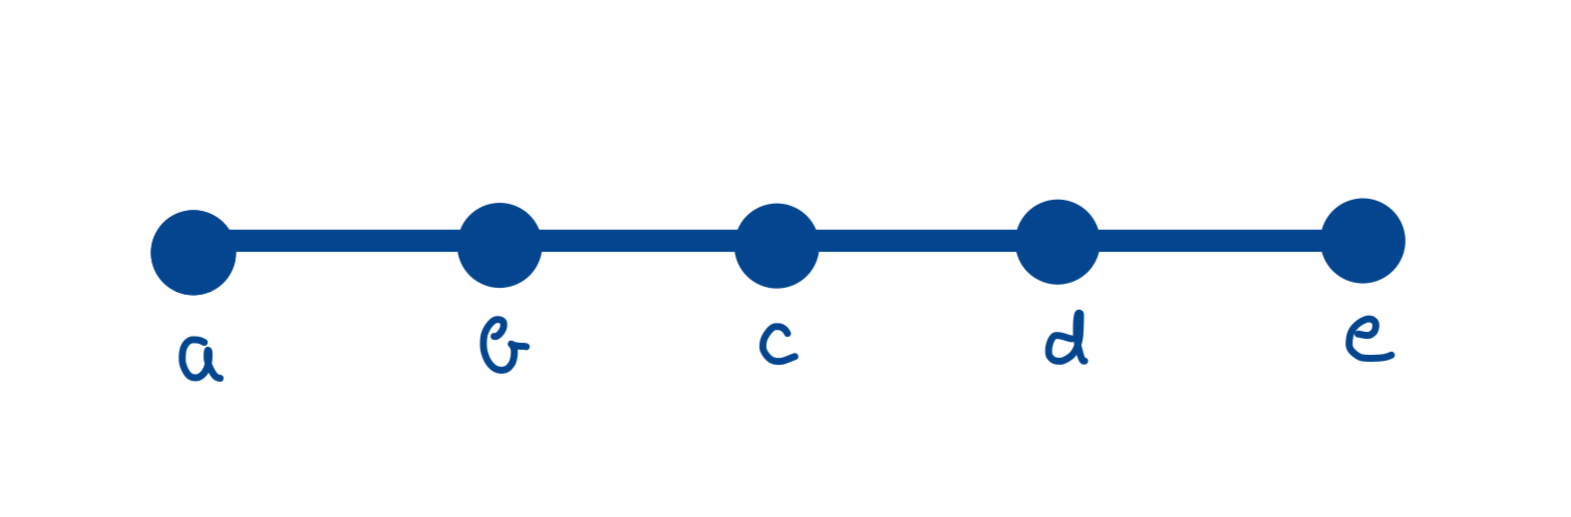
\includegraphics[width=0.6\textwidth]{pot.jpg}      
\end{figure}

\end{primer}

\begin{primer}\label{primer_2.5.}
    Cikel dolžine $n$ označujmo z $C_n$. Vozlišča označimo z $v_1, v_2, ..., v_n$, kot 
    je prikazano na spodnji sliki. Izberimo podmnožico $W = {v_1, v_2} \subseteq V(G).$ 
    Metrične predstavitve vozlišč grafa $C_n$, glede na izbrano podmnožico vozlišč, so potem sledeče:
    \begin{align*}
        r_W(v_1) = (d(v_1, v_1), d(v_1, v_2)) & = (0, 1) \\
        r_W(v_2) = (d(v_2, v_1), d(v_2, v_2)) & = (1, 0) \\
        r_W(v_3) = (d(v_3, v_1), d(v_3, v_2)) & = (2, 1) \\
        r_W(v_4) = (d(v_4, v_1), d(v_4, v_2)) & = (3, 2) \\
        & \dots \\
        r_W(v_{n-1}) = (d(v_{n-1}, v_1), d(v_{n-1}, v_2)) & = (2, 3) \\
        r_W(v_n) = (d(v_n, v_1), d(v_n, v_2)) & = (1, 2)
    \end{align*}
    
    Zopet vidimo, da so metrične predstavitve vseh vozlišč med seboj različne.
    $W$  je torej rešljiva množica, njena velikost pa je enaka $2$. Metrična dimenzija
    poljubno velikega cikla je enaka $\beta(C_n) = 2.$

    \begin{figure}[h]
        \caption{Graf $C_5$.}
        \centering
        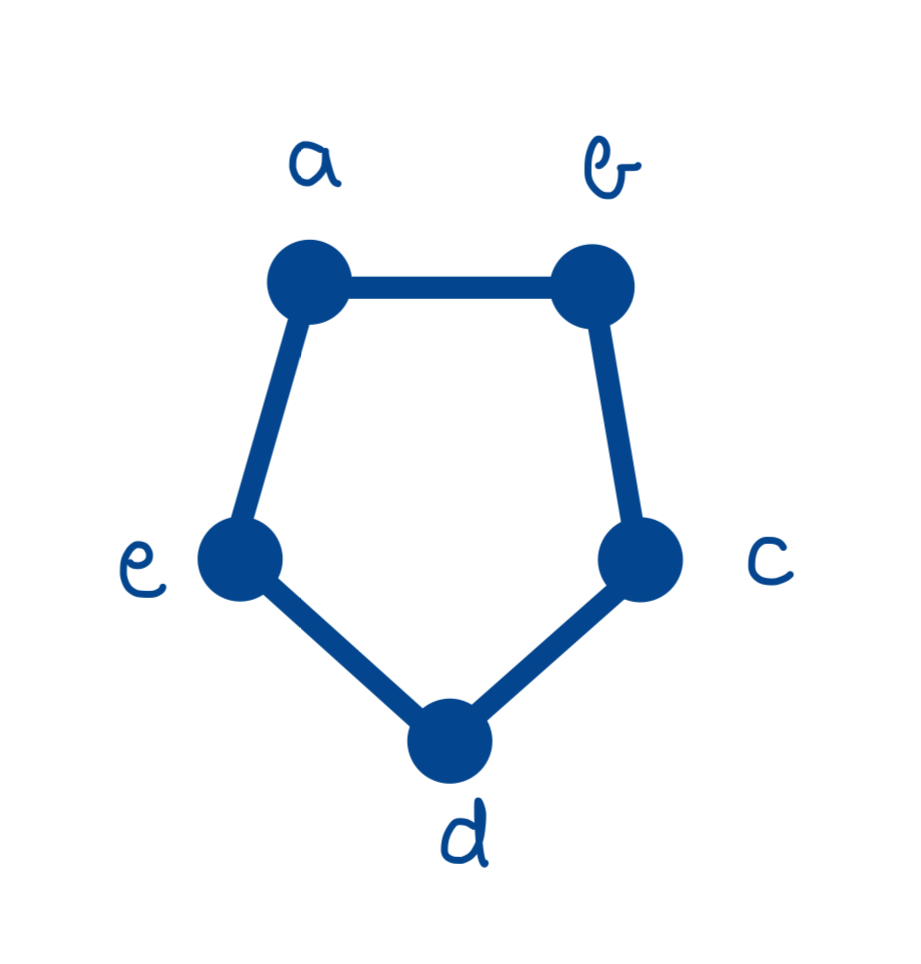
\includegraphics[width=0.4\textwidth]{cikel.jpg}
    \end{figure}
%te sklice še popravi oznake
\end{primer}




\subsection{Lastnosti}

Nekaj osnovnih ugotovitev o rešljivih množicah grafa lahko razberemo iz zgornjih primerov.

\begin{trditev}
Za povezan graf $G$, je $V(G)$ rešljiva množica.
\end{trditev}
\begin{dokaz}
Predpostavimo, da ima graf $G$ $n$ vozlišč. Označimo vozlišča grafa $G$ z $v_1, ..., v_n$.
Za posamezno vozlišče bo metrična predstavitev sledeča:
$$r_{V(G)}(v_k) = (d(v_k, v_1), ..., d(v_k, v_k), ... , d(v_k, v_n)) = (d(v_k, v_1), ..., 0 , ... , d(v_k, v_n)).$$
Torej za vsako vozlišče $v_k$ bo $k$-ta komponenta metrične predstavitve enaka $0$. To je tudi edina komponenta v vektorju, 
ki bo enaka $0$, saj za razdaljo med vozlišči velja
$$d(v, w) = 0 \Leftrightarrow v = w.$$
Sledi $\forall u, v \in V(G): u \neq v \implies r_{V(G)}(v) \neq r_{V(G)}(u)$, torej je $V(G)$ rešljiva množica.
\end{dokaz}

% a je sploh definirana razdalja na nepovezanem grafu?? s bi se dalo narest kakšno smiselno razširitev??
%iz te trditve sledi, da metrična dimenzija vselej obstaja in je manjša ali enaka |V(G)|.

\begin{trditev}
    Rešljiva baza grafa $G$ ni enolično določena.
\end{trditev}
\begin{dokaz}
    To hitro vidimo na primeru %\ref*{primer_2.4.}.
    Za $W$ bi lahko vezli tudi vozlišče $v_2$ in prišli do enakega rezultata.
\end{dokaz}

V defnicijah 2.1. in 2.2. smo prepostavili, da imamo neprazno podmnožico vozlišč. Če bi vzeli prazno množico,
bi bila definicija očitno nesmiselna. Iz trditve 2.6. lahko potem sklepamo, da metrična dimenzija za graf vselej 
obstaja in lahko zapišemo naslednjo posledico:

\begin{posledica}
    Za povezan graf $G$ velja 
    $$1 \leq \beta(G) \leq |V(G)| - 1. $$
\end{posledica}
\begin{dokaz}
    Iz definicije metrične dimenzije sledi $1 \leq \beta(G)$. Iz trditve 2.6. pa sledi $\beta(G) \leq |V(G)|.$
    Predpostavimo $|V(G)| = n$ in $V(G) = \{ v_1, ... , v_n\}$. Vzemimo sedaj podmnožico $W = \{ v_1, ... , v_{n-1}\}.$
    Metrične predstavitve vozlišč glede na $W$ so sledeče:

    \begin{align*}
        r_W(v_1) & = (0, d(v_1, v_2), ..., d(v_1, v_k), ... , d(v_1, v_{n-1})) \\
        r_W(v_2) & = (d(v_2, v_1), 0, ..., d(v_2, v_k), ... , d(v_2, v_{n-1})) \\
        & \dots \\
        r_W(v_k) & = (d(v_k, v_1), d(v_k, v_2), ..., 0 , ... , d(v_k, v_{n-1})) \\
        & \dots \\
        r_W(v_{n-1}) & = (d(v_{n-1}, v_1), d(v_{n-1}, v_2), ... , d(v_{n-1}, v_k) , ..., 0) \\
        r_W(v_n) & = (d(v_n, v_1), d(v_n, v_2), ...,  d(v_n, v_k), ... , d(v_n, v_{n-1})) \\
    \end{align*}
    Vidimo, da so vse metrične predstavitve med seboj različne, torej je $W$ rešljiva in $\beta(G) \leq n - 1.$ 
\end{dokaz}

%Konec koncev je vsega konec.%
%Začetki so najtežji.%

\subsubsection{Metrična dimenzija in premer grafa}

Ni presenetljivo, da lahko najdemo povezavo med metrično dimenzijo in premerom grafa.
Spomnimo se matematične definicije premera.

\begin{definicija}
    Premer grafa $G$ označujemo z ${\rm diam}(G)$ in je enak dolžini najdaljše najkrajše poti v grafu.
    Torej $${\rm diam}(G) = \underset{v, u \in V(G)}{\max} d(u, v).$${{}}
\end{definicija}

\begin{trditev}
    Naj bo $G$ povezan graf in $|V(G)| = n$. Potem velja naslednja povezava:
    $$n \leq ({\rm diam}(G))^{\beta (G)} + \beta (G). $$
\end{trditev}

\begin{dokaz}
    Naj bo $R$ rešljiva baza grafa $G$, torej $|R| = \beta(G).$ Zanima nas, največ koliko vozlišč
    ima lahko tak graf $G$. Vozlišča iz množice $R$ bodo imela natanko eno komponento metrične predstavitve
    enako nič, tako se bodo te razlikovale med sabo in vseh ostalih. 
    Če pa vzamemo vozlišče $v \notin R$, pa velja sledeče:
    $$\forall r_i \in R: 1 \leq d(v, r_i) \leq {\rm diam}(G).$$
    
    Vseh možnih različnih metričnih predstavitev za vozlišča izven rešljive množice $R$ 
    je tako $({\rm diam}(G))^{\beta (G)}$
    in lahko zapišemo:
    $$n \leq ({\rm diam}(G))^{\beta (G)} + \beta (G).$$
\end{dokaz}

V resnici lahko red grafa z dano metrično dimenzijo in premerom še bolj omejimo.

\begin{trditev}
    Naj bo $G$ povezan graf in $|V(G)| = n$. Označimo $ \delta = {\rm diam}(G)$ in $\beta = \beta (G)$. 
    Potem velja

    $$n \leq \Bigl ( \Bigl \lfloor {\frac{2 \delta}{3}}\Bigr \rfloor + 1 \Bigr )^{\beta} + 
    \beta \sum_{i = 1}^{\lceil D/3 \rceil} {(2i - 1)^{\beta - 1}}. $$
\end{trditev}

\begin{dokaz}
    
\end{dokaz}

Ta zgornja meja postane še bolj natančna za posamezne družine grafov, vendar v tem delu
tega ne bomo obravnavali tako podrobno.

\subsubsection{Dvojčki in metrična dimenzija}
Spomnimo se pojma soseščine vozlišča.

\begin{definicija}
    Naj bo $G$ povezan graf in $v \in V(G)$ vozlišče na grafu. Množico 
    $$N(v) = \{u \in V(G) \, | \,vu \in E(G) \}$$ imenujemo soseščina vozlišča $v$.
\end{definicija}

Sedaj vpeljimo ekvivalenčno relacijo na vozliščih
$$v \equiv u \Leftrightarrow N(v)\setminus \{u\} = N(u) \setminus \{v\}$$
Če sta vozlišči v tej ekvivalenčni relaciji, pravimo, da sta dvojčka. 
Ekvivalenčni razred vozlišča $v$ označimo z $v^{*}$, 
množico vseh ekvivalenčnih razredov z $\tau (G)$, število vseh razredov pa naj bo označeno 
z $|\tau(G)| = \iota(G).$

\begin{lema}
    Naj bosta $u, v \in v(G)$ dvojčka. Potem je 
    $$\forall w \in V(G) \setminus \{u, v\} : d(u, w) = d(v, w).$$
\end{lema}

\begin{dokaz}
    %napiši dokaz
\end{dokaz}

Iz tega sledi, da mora vsaka rešljiva množica vsebovati vsaj enega od dvojčkov.
Zapišemo lahko naslednjo trditev:

\begin{trditev}
    Za povezan graf $G$ velja
    $$\beta(G) \geq \sum_{v^{*} \in \tau(G)} (|v^{*}| - 1).$$
\end{trditev}

\begin{dokaz}
    % napiši dokaz
\end{dokaz}

%%%%%%%%%%%%%%%%%%%%%%%%%%%%%%%%%%%%%%%%%%%%%%%%%%%%%%%%%%%%%
%%%%%%%%%%%%%%%%%%%%%%%%%%%%%%%%%%%%%%%%%%%%%%%%%%%%%%%%%%%%%
\section{Leksikografski produkt grafov}



\begin{definicija}
    Leksikografski produkt $G[H]$ grafov $G$ in $H$ je definiran na množici vozlišč $V (G[H]) = V (G)\times V (H)$. Dve različni vozlišči $(u, v)$ in $(x, y)$ sta sosedni, kadar velja
\begin{itemize}
    \item $ux \in E(G)$ ali
    \item $u = x$ in $vy \in E(H).$ 
\end{itemize}
\end{definicija}

%%%%%%%%%%%%%%%%%%%%%%%%%%%%%%%%%%%%%%%%%%%%%%%%%%%%%%%%%%%%%%%%%%%%%%%%%%%%%%
\subsection{primer}
Za lažjo predstavo si lahko ogledamo spodnjo skico, ki prikazuje leksikografski produkt
dveh naključnih povzeanih grafov.
\begin{figure}[h]
    \caption{Leksikografski produkt poljubnih povezanih grafov $G$ in $H$.}
    \centering
    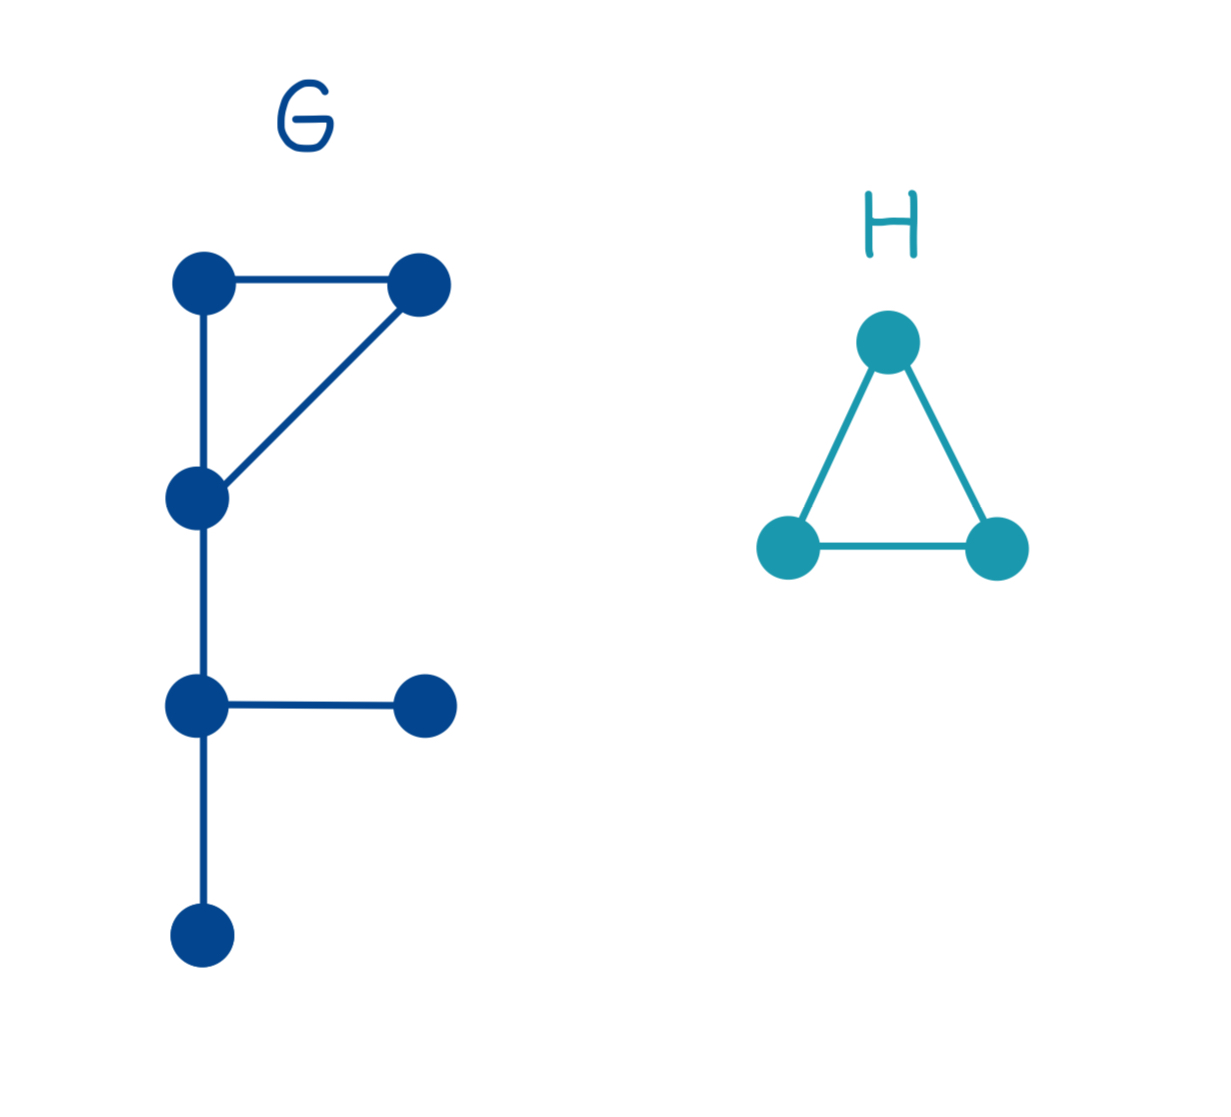
\includegraphics[width=0.5\textwidth]{leks_produkt_1.jpg}
    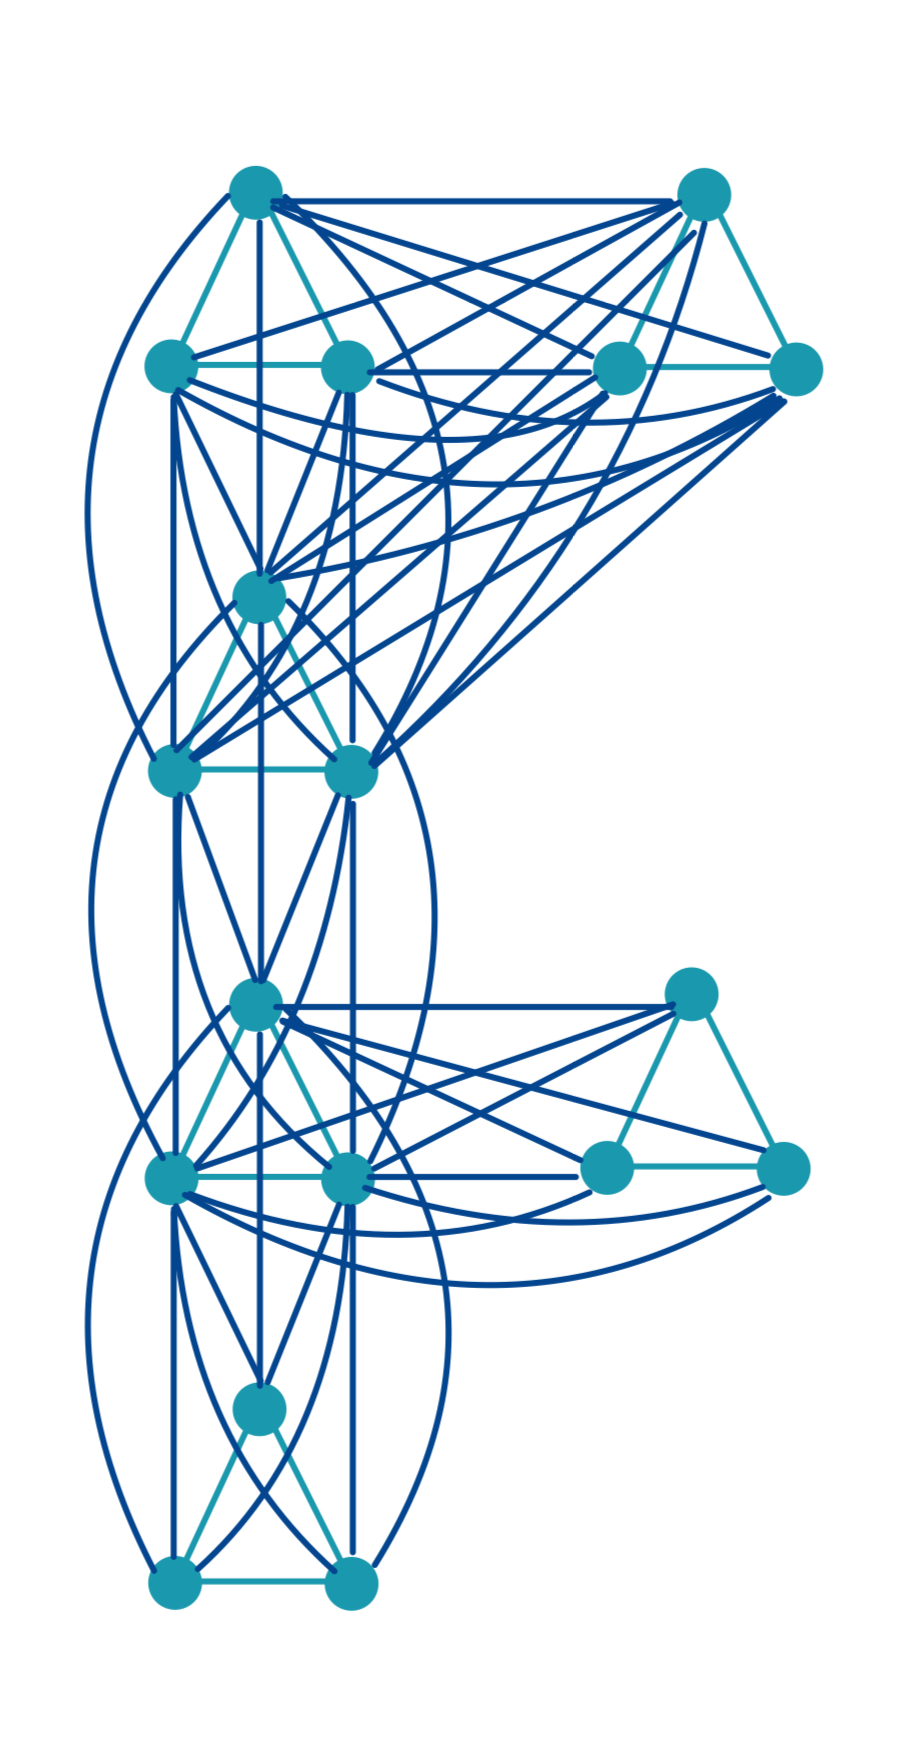
\includegraphics[width=0.2\textwidth]{leks_produkt_2.jpg}        
\end{figure}

%%%%%%%%%%%%%%%%%%%%%%%%%%%%%%%%%%%%%%%%%%%%%%%%%%%%%%%%%%%%%%%%%%%%%%%%%%%%%%


\subsection{lastnosti}
Nekaj osnovnih lastnosti leksikografskega produkta grafov:
\begin{itemize}
    \item POVEZANOST: Če je $G$ povezan graf, potem je $G[H]$ povezan. 
    \item NEKOMUTATIVNOST: v splošnem velja $G[H] \neq H[G].$
    \item DISTRIBUTIVNOST: $(G_1 + G_2)[H] = G_1[H] + G_2[H],$ kjer $+$ označuje disjunktno unijo oz. vsoto grafov.
    %definiraj vsoto grafov...
    \item ENAKOST KOMPLEMENTOV: $\overline{G[H]} = \overline{G} [\overline{H}].$
    % kako bi se v resnici pravilno reklo tej lastnosti...?
\end{itemize}

Poglejmo si kako izgleda razdalja med vozliščema v leksikografskem prodkutu grafov. 
Označimo preslikavo  $a: V(G) \times V(G) \rightarrow \mathbb{N};$   
$$ a(v, w) = \begin{cases}
    0; & v = w \\
    1; & v \sim w \\
    2; & v \not\sim w
\end{cases} 
$$ 
Opazujemo Leksikografski produkt povezanega grafa $G$ reda $n$, z množico vozlišč
$V(G) = \{v_1, v_2, ... , v_n \}$ in grafa $H$ reda $m$, z množico vozlišč 
$V(H) = \{u_1, u_2, ... , u_m \}$. Zaradi boljše preglednosti vpeljimo oznako $v_{ij} := (v_i, u_j) \in V(G[H]).$
Sedaj lahko zapišemo
$$
d_{G[H]}(v_{ij}, v_{rs}) = \begin{cases}
        d_G(v_i, v_r); & v_i \neq v_r \\
        a_H(u_j, u_s); & \text{sicer}
    \end{cases}
$$ 

%%%%%%%%%%%%%%%%%%%%%%%%%%%%%%%%%%%%%%%%%%%%%%%%%%%%%%%%%%%%
%%%%%%%%%%%%%%%%%%%%%%%%%%%%%%%%%%%%%%%%%%%%%%%%%%%%%%%%%%%%
\section{Metrična dimenzija leksikografskega produkta grafov}
Decembra leta 2010 sta v razmaku 17 dni nastala dva različna članka na temo metrične dimenzije leksikografskega produkta grafov. 
Avtorji so se lotili teme s povsem različnima pristopoma, v tem diplomskem seminarju pa bomo povzeli rezultate obeh in poskusili poiskati povezavo med njimi.  

\subsection{Metrična dimenzija in komponente}


\subsection{Metrična dimenzija, sosedska dimenzija in dvojčki}

\subsection{Povezave in skupni rezultati??}
%če mi to rata sem car.


% \section{...}
% ...

% \section{Zaključek}
% ...

\end{document}
